% Данный файл распространяетсяя под лицензией CC BY 4.0. Текст лицензии размещён на https://creativecommons.org/licenses/by/4.0/
% (c) Кафедра системного программирования, 2025

\documentclass[a4paper]{article}

\usepackage[a4paper, top=8mm, bottom=8mm, left=8mm, right=8mm]{geometry}

\usepackage[english,russian]{babel}
\usepackage{fontspec}

%\usepackage{fontspec}
\setmainfont{FreeSerif}
\setsansfont{FreeSans}
\setmonofont{FreeMono}

\usepackage[tiny, compact]{titlesec}

\usepackage{titling}
\setlength{\droptitle}{-1cm}
\pretitle{\begin{center}\begin{bfseries}\Large}
\posttitle{\par\end{bfseries}\end{center}}
\preauthor{\begin{center}\normalsize}
\postauthor{\par\end{center}\vspace{-1.8cm}}

\usepackage{hyperref}
\usepackage{bookmark}
\usepackage{csquotes}
% Сюда можно дописывать нужные вам пакеты.
\usepackage{float} 
\usepackage{graphicx}      
\usepackage{caption}       
\usepackage{subcaption}    

\title{Реализация алгоритма Борувки поиска минимального остовного дерева, с использованием
библиотеки Spla}

\author{Угарова Полина Павловна}

% Дата много места занимает, её лучше не указывать.
\date{}

\begin{document}

\maketitle

\begin{flushright}
    Группа: \enquote{2025.Б73-мм}

    Кафедра: \emph{кафедра Системного программирования}

    % Степень/звание и должность научника мы лучше вас знаем, их можно не указывать.
    Научный руководитель: \emph{Григорьев Семен Вячеславович}

    % А вот про консультанта укажите официальное место работы, с "ООО" или чем-то таким, и должностью желательно по трудовой, не просто "techlead". Выясните у консультанта.
    Консультант: \emph{Кутуев Владимир Александрович}
    
    Старший инженер-исследователь YADRO
    
    Номер семестра практики: \emph{2}
\end{flushright} 

\section{Введение}
Библиотека Spla \cite{spla_orig, orachev} --- это библиотека обобщенной разреженной линейной алгебры с открытым исходным кодом и по на графических процессорах (GPGPU). Использование OpenCL (Open Computing Language) --- открытого стандарта для написания программ, которые используют параллельные вычисления на различных устройствах --- позволяет Spla работать на GPGPU различных производителей, а также на многоядерных процессорах. Spla использует идеи GrpahBLAS \cite{graphblas} и нацелена на разработку алгоритмов анализа графов.
\section{Постановка задачи}

В рамках проекта по развитию библиотеки \textbf{SPLA (Sparse Linear Algebra)} уже реализован набор алгоритмов анализа графов, содержащий такие алгоритмы, как обход в ширину (BFS) и PageRank. Однако в библиотеке отсутствует алгоритм для поиска минимального остовного дерева (Minimum Spanning Tree), который и был реализован в рамках данной работы.

Для реализации был выбран \textbf{алгоритм Борувки}, так как он предоставляет естественные возможности для параллельной реализации через операции линейной алгебры, поддерживаемые SPLA.

В ходе работы необходимо решить следующие \textbf{задачи}:

\begin{enumerate}
    \item \textbf{Поддержка нового скалярного типа} в SPLA --- пары из номера вершины и веса ребра (\texttt{Pair}), необходимой для работы со взвешенными графами.
    
    \item \textbf{Реализация операций над типом \texttt{Pair}}, образующих полукольцо:
    \begin{itemize}
        \item[$\oplus$] \textbf{сложение/минимум}: выбор пары с минимальным весом. При равенстве весов выбирается пара с меньшим номером вершины.
        \[
        \min((w_1, v_1), (w_2, v_2))
        \]
        \item[$\otimes$] \textbf{умножение/комбинирование}: комбинирование, которое берёт вес из первой пары, а вершину --- из второй.
        \[
        (w_1, v_1) \otimes (w_2, v_2) = (w_1, v_2)
        \]
    \end{itemize}
    
    \item \textbf{Реализация алгоритма Борувки} с использованием операции умножения разреженной матрицы на вектор (\texttt{mxv}) на основе введённого полукольца.
    
    \item \textbf{Интеграция реализованного алгоритма} в экосистему SPLA с поддержкой GPU-ускорения через OpenCL.
    
    \item \textbf{Тестирование и верификация} алгоритма на тестовых графах, включая замер производительности.
\end{enumerate}

Результаты работы необходимы для расширения функциональности библиотеки SPLA в области графовых алгоритмов. Для конечных пользователей продукта это полезно возможностью эффективного построения минимального остовного леса на GPU. 

\section{Описание предлагаемого решения}

Основная идея решения заключается в использовании \textbf{полукольцевой структуры} для элегантной реализации алгоритма Борувки через операцию умножения разреженной матрицы на вектор (\texttt{mxv}). Алгоритм Борувки был выбран, поскольку каждая его итерация может быть выполнена параллельно: все компоненты графа независимо выбирают минимальное исходящее ребро.

\textbf{Ключевые этапы алгоритма:}
\begin{enumerate}
    \item Для каждой вершины выбирается минимальное инцидентное ребро (с учётом текущей принадлежности к компонентам)
    \item Для каждой компоненты из выбранных рёбер остаётся только минимальное
    \item Выбранные рёбра добавляются в минимальное остовное дерево
    \item Компоненты сливаются в одну
    \item Процесс повторяется до тех пор, пока не останется одна компонента
\end{enumerate}

\begin{table}[H]
\centering
\begin{tabular}{|p{3cm}|p{4cm}|p{4cm}|}
\hline
\textbf{Подход} & \textbf{Преимущества} & \textbf{Недостатки} \\
\hline
Алгоритм Крускала & Простота реализации & Плохо параллелизуется, требует сортировки рёбер \\
\hline
Алгоритм Прима & Хорош для плотных графов & Последовательный, сложно распараллелить \\
\hline
\textbf{Алгоритм Борувки} (предлагаемое решение) & Естественно параллелизуется, $O(E \log V)$ & Требует поддержки операций над компонентами \\
\hline
\end{tabular}
\caption{Сравнение алгоритмов построения минимального остовного дерева}
\end{table}

В отличие от классических реализаций, в данной работе алгоритм выражается через операции линейной алгебры, что позволяет использовать готовые оптимизированные ядра SPLA и выполнять вычисления на GPU. Аналогичные подходы существуют в библиотеке \textbf{GraphBLAS}, но SPLA предоставляет более гибкую систему типов и поддержку различных бэкендов (OpenCL, CPU).

Интеграция с существующей кодовой базой SPLA потребовала:
\begin{itemize}
    \item добавления нового типа в систему типов библиотеки;
    \item регистрации новых операций в CPU и OpenCL бэкендах;
    \item модификации генератора OpenCL-кода для поддержки пользовательских типов.
\end{itemize}


В рамках работы предложено реализовать алгоритм Борувки через полукольцевую структуру \texttt{combMin}, что позволяет свести его к операции \texttt{mxv} и эффективно выполнять на GPU. В отличие от классических последовательных алгоритмов (Крускала, Прима), выбранный подход обеспечивает естественный параллелизм. Для поддержки взвешенных графов в библиотеку SPLA был добавлен новый тип \texttt{Pair} (вес + вершина), а также операции минимума и комбинирования, образующие полукольцо. Реализация выполнена на C++17 с использованием OpenCL для GPU-ускорения. Интеграция с SPLA потребовала расширения системы типов и модификации генератора OpenCL-кода.
\section{Эксперименты}
\subsection{Цель экспериментов}

Целью экспериментов являлась проверка корректности реализованного алгоритма Борувки, а также оценка его производительности в двух аспектах:
\begin{enumerate}
    \item сравнение с оптимизированной библиотекой LAGraph \cite{lagraph} на платформе RISC-V;
    \item детальный профайлинг шагов итерации алгоритма для выявления узких мест.
\end{enumerate}

\subsection{Среда проведения экспериментов}
Измерения производительности проводились с использованием библиотеки \textbf{graph-bench} \cite{graphbench}. Для каждого графа выполнялось по 5 запусков алгоритма, в качестве итогового результата бралось среднее арифметическое время выполнения.

Для профайлинга шагов алгоритма (выявление узких мест) выполнялcя запуск на ноутбуке с замером времени каждого логического шага итерации.

Эксперименты проводились на двух различных платформах.

\begin{table}[H]
\centering
\begin{tabular}{|p{4cm}|p{4cm}|p{4cm}|}
\hline
\textbf{Компонент} & \textbf{Платформа 1 (RISC-V)} & \textbf{Платформа 2 (ноутбук)} \\
\hline
GPU(OpenCL Devices) & (PowerVR) PowerVR B-Series, \newline (Clover) AMD CAICOS, \newline (PoCL) SpacemiT X60 & Intel UHD Graphics \\
\hline
\end{tabular}
\caption{Конфигурация тестовых платформ}
\end{table}
\subsection{Сравнение производительности с LAGraph на RISC-V}

\begin{figure}[H]
\centering
\begin{subfigure}{0.45\textwidth}
    \centering
    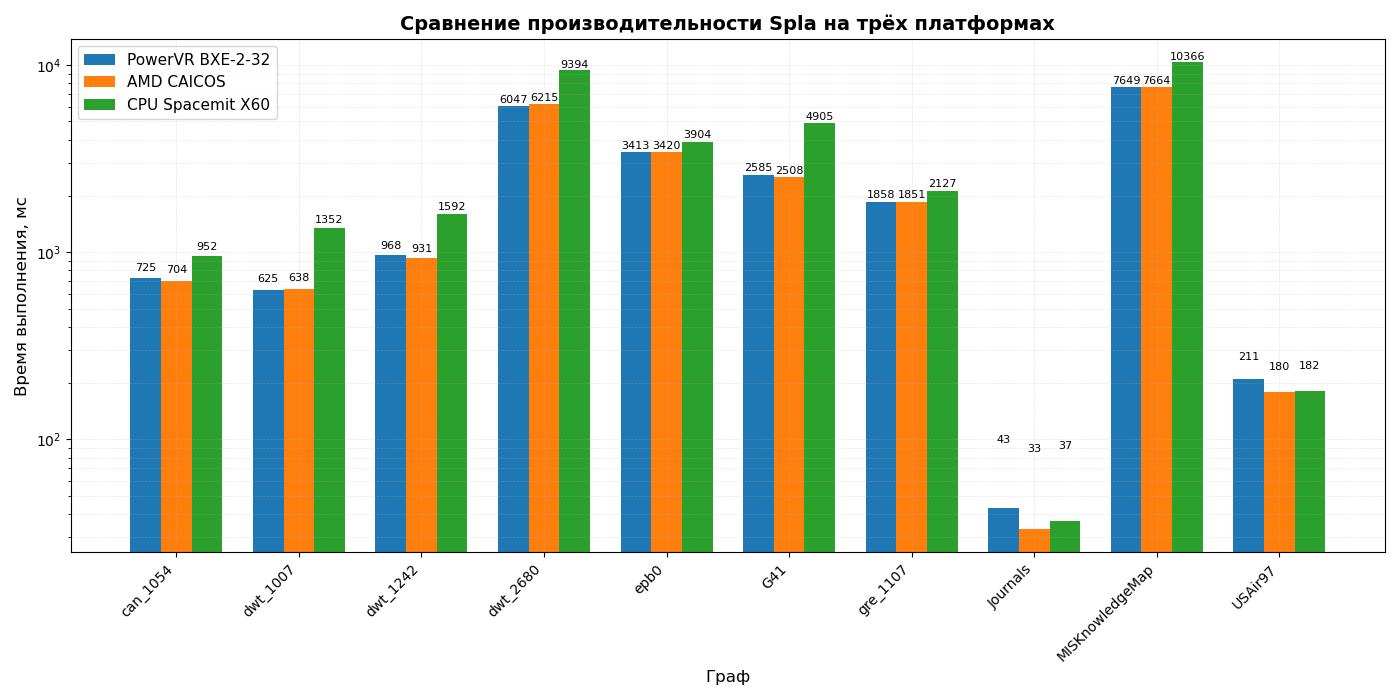
\includegraphics[width=\textwidth]{figures/Figure_1.png}
\end{subfigure}
\hfill
\begin{subfigure}{0.45\textwidth}
    \centering
    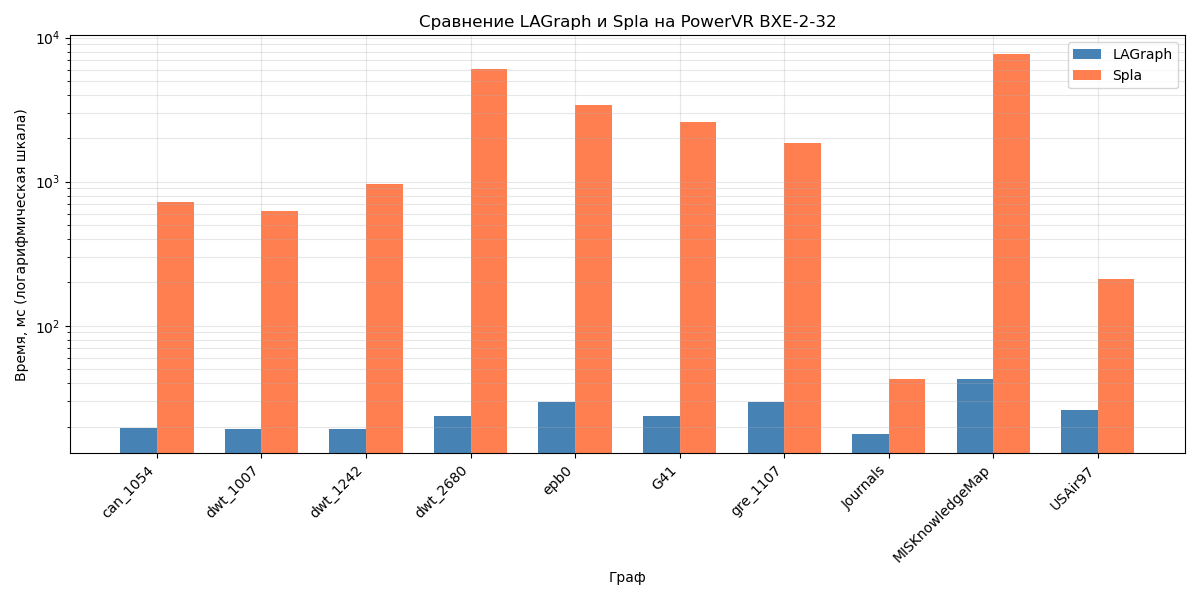
\includegraphics[width=\textwidth]{figures/Figure_2.png}
\end{subfigure}
\label{fig:comparison}
\caption{Сравнения времени выполнения алгоритма на разных opencl платформах на RISC-V и с LAGraph реализацией)}
\end{figure}

\subsubsection*{Выводы}

\begin{enumerate}
    \item SPLA успешно использует параллелизм GPU на всех тестовых графах;
    \item Алгоритм \textbf{корректно} работает на всех тестовых графах;
    \item Реализация \textbf{переносима} между разными OpenCL-платформами (PowerVR GPGPU, AMD GPGPU, многоядерный RISC-V CPU);
    \item Наблюдается существенное отставание от оптимизированной LAGraph реализации (в 30–260 раз).
\end{enumerate}

Основной причиной низкой производительности предложенного решения по сравнению с LAGraph является \textbf{недостаточный набор эффективных примитивов} для работы с матрицами и векторами в SPLA, что открывает направления для дальнейшей работы.
\subsection{Анализ узких мест}

\begin{figure}[H]
\centering
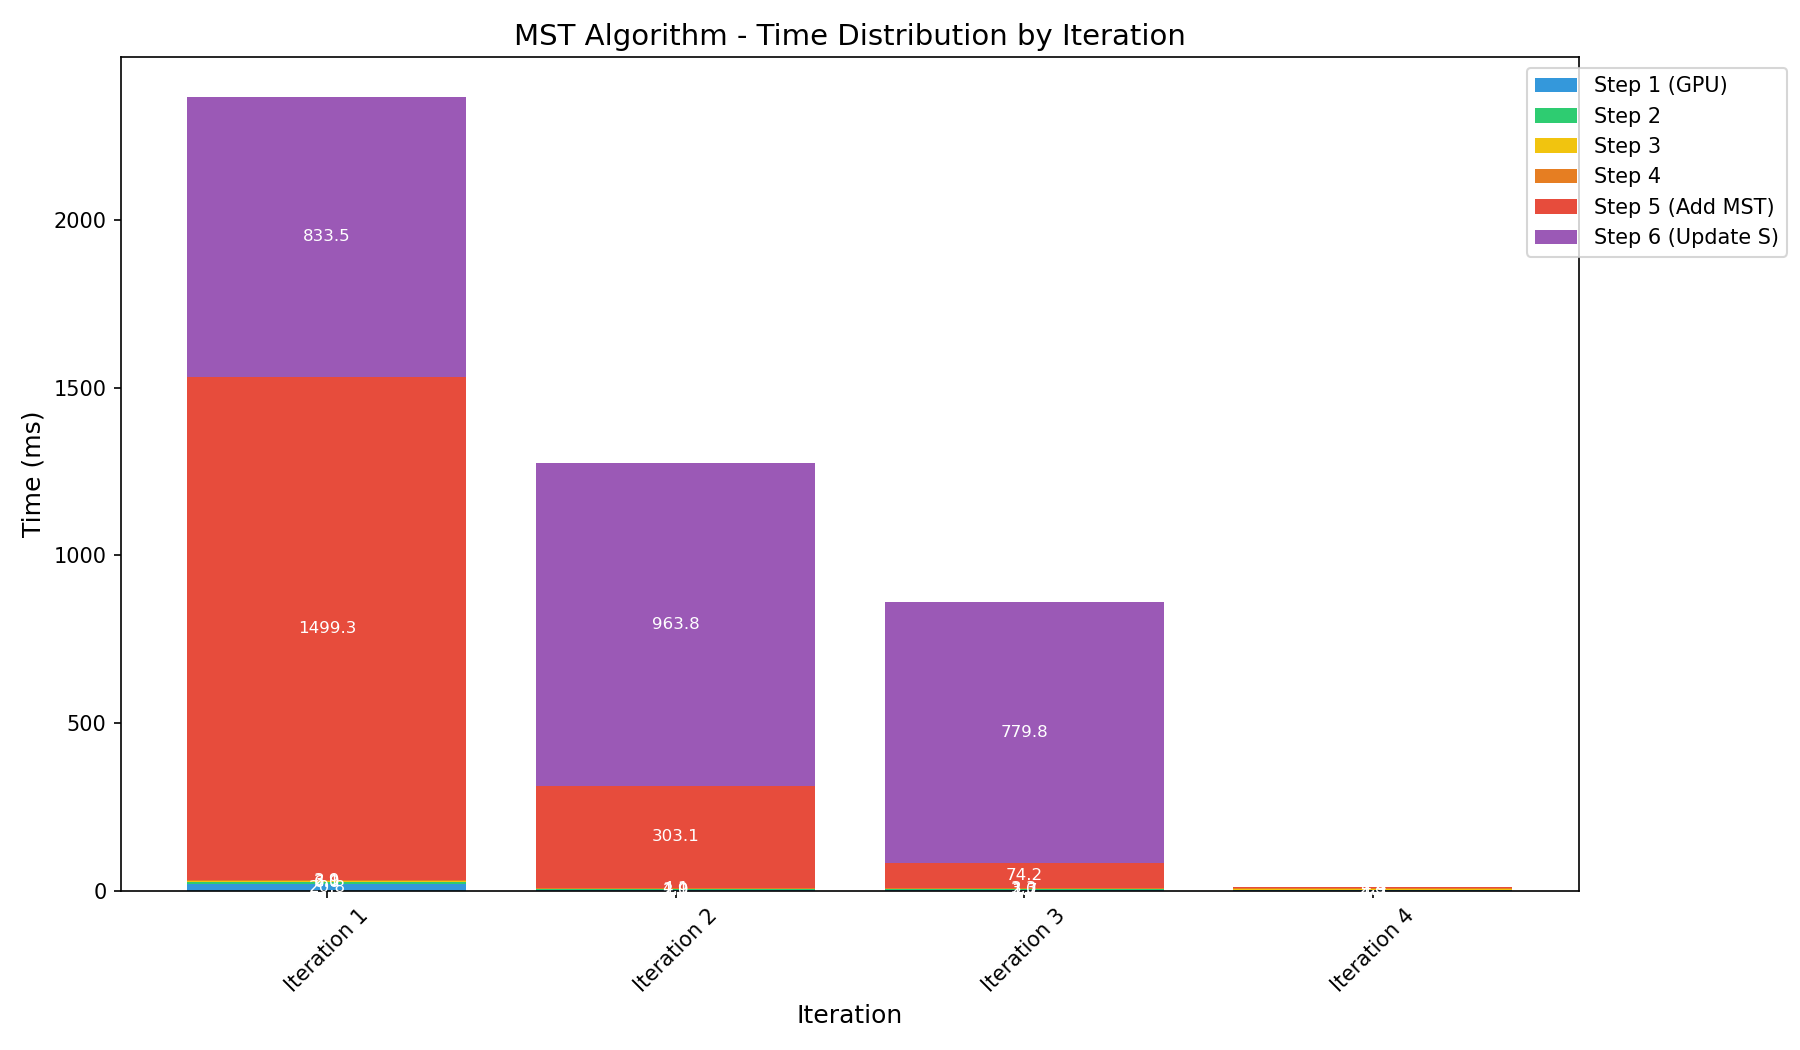
\includegraphics[width=0.5\textwidth]{figures/image.png}
\caption{Время выполнения каждого шага внутри каждой итерации алгоритма)}
\end{figure}

\subsubsection*{Выводы}

\begin{enumerate}
    \item \textbf{Основная проблема производительности} — шаги 5 и 6, на которые приходится более 95\% времени выполнения (4448 мс из 4571 мс общего времени).
    
    \item \textbf{Причина}: в SPLA отсутствуют GPU-функции для:
    \begin{itemize}
        \item параллельного добавления рёбер в матрицу МОД (Step 5);
        \item параллельной фильтрации внутрикомпонентных рёбер и обновления компонент (Step 6).
    \end{itemize}
    
    \item \textbf{Итеративный характер}: эти операции выполняются последовательно на CPU и повторяются на каждой итерации алгоритма, что сводит на нет преимущества GPU-ускорения на ранних шагах.
    
    \item \textbf{Направление для оптимизации}: реализация параллельных версий Step 5 и Step 6 на GPU позволит значительно сократить общее время выполнения алгоритма.
\end{enumerate}

\subsection{Апробация}

Результаты работы были представлены:
\begin{itemize}
    \item в виде Pull Request в репозиторий SPLA \item \textbf{Pull Request:} \url{https://github.com/SparseLinearAlgebra/spla/pull/241}
\end{itemize}
\section{Заключение}

В ходе выполнения работы получены следующие результаты:

\begin{enumerate}
    \item \textbf{Новый тип данных:} в библиотеку SPLA добавлен скалярный тип \texttt{Pair} (вес ребра + номер вершины), необходимый для работы со взвешенными графами.
    
    \item \textbf{Операции полукольца:} реализованы операции $\oplus$ (выбор пары с минимальным весом) и $\otimes$ (комбинирование), образующие полукольцо \texttt{combMin}, позволяющее выразить алгоритм Борувки через умножение матрицы на вектор.
    
    \item \textbf{Алгоритм Борувки:} реализован алгоритм построения минимального остовного дерева с использованием примитивов SPLA и GPU-ускорением через OpenCL.
    
    \item \textbf{Тестирование:} проведена верификация алгоритма на тестовых графах, написаны тесты на операции пары.
    
    \item \textbf{Сравнительный анализ:} произведено сравнение производительности с библиотекой LAGraph на платформе RISC-V, выявлено отставание в 30–260 раз, обусловленное недостаточной оптимизацией примитивов SPLA.
\end{enumerate}

Решение не является финальным и открывает направления для дальнейшей работы:
\begin{itemize}
    \item реализация GPU-функций для шагов 5 и 6 алгоритма (добавление рёбер и фильтрация компонент);
    \item оптимизация примитивов SPLA для сокращения отставания от LAGraph.
\end{itemize}
\begin{thebibliography}{99}
\bibitem{spla_orig} Исходный код библиотеки Spla [Электронный ресурс]. URL: https://github.com/SparseLinearAlgebra/spla
\bibitem{orachev} Орачев Е. Generalized sparse linear algebra library with vendor-agnostic GPUs acceleration. URL: https://dspace.spbu.ru/items/2aa43d43-60f5-465d-981d-a8078c69297c
\bibitem{graphblas} Buluç A. et al. Design of the GraphBLAS API for C // 2017 IEEE IPDPSW. — С. 643-652.
\bibitem{graphbench} Исходный код библиотеки graph-bench. URL: https://github.com/EgorOrachyov/graph-bench
\bibitem{lagraph} Исходный код библиотеки LAGraph. URL: https://github.com/GraphBLAS/LAGraph
\end{thebibliography}
\end{document}